\documentclass[11pt]{beamer}
\usetheme{CambridgeUS}
\usepackage[utf8]{inputenc}
\usepackage[spanish]{babel}
\usepackage{amsmath}
\usepackage{amsfonts}
\usepackage{amssymb}
\author{Definición y propiedades}
\title{Integral de Riemann-Stieltjes}
%\setbeamercovered{transparent}
%\setbeamertemplate{navigation symbols}{}
%\logo{}
%\institute{}
%\date{}
%\subject{}
\begin{document}

\begin{frame}
\titlepage
\end{frame}

% \begin{frame}
% \tableofcontents
% \end{frame}

\begin{frame}{Particiones}

\begin{definition}
Sea $[a, b]$ intervalo. Una \textit{partición} de $[a, b]$ es un conjunto de puntos $x_0, x_1,..., x_n$ tales que
\begin{equation*}
	a = x_0 \leq x_1 \leq \dots \leq x_n = b
\end{equation*}
Sean
\begin{equation*}
	\Delta x_i = x_i - x_{i-1} (i = 1, \dots, n)
\end{equation*}
\end{definition}

\begin{center}
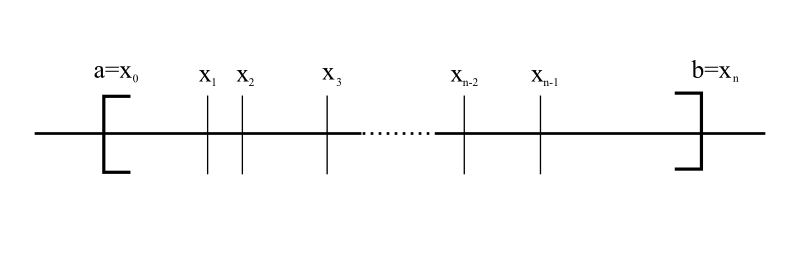
\includegraphics[scale=1]{img/particion.png}
\end{center}

\end{frame}

\begin{frame}{Integral de Riemann}

Sea $f$ es una función real acotada definida en $[a, b]$. Para cada partición $P$ de $[a, b]$ definimos

\begin{equation*}
	\begin{array}{rcll}
		M_i & = & \sup f(x) & (x_{i-1} \leq x \leq x_i), \\
		m_i & = & \inf f(x) & (x_{i-1} \leq x \leq x_i), \\
		U(P, f) & = & \sum_{i=1}^n M_i \Delta x_i , \\
		L(P, f) & = & \sum_{i=1}^n m_i \Delta x_i
	\end{array}
\end{equation*}
y finalmente
\begin{equation}
	\begin{array}{rcl}
		\bar{\int}_a^b f\,dx & = & \inf U(P, f)
	\end{array}
\end{equation}
\begin{equation}
	\begin{array}{rcl}
		\underline{\int}_a^b f\,dx & = & \sup L(P, f)
	\end{array}
\end{equation}

Las partes izquierdas de estas ecuaciones son llamadas \textit{integral superior} e \textit{integral inferior} de $f$ sobre $[a, b]$ respectivamente.

\end{frame}

\begin{frame}{Integral de Riemann}

Si las integrales \textit{superior} e \textit{inferior} son iguales entonces decimos que $f$ es \textit{riemann-integrable} en $[a, b]$ y diremos que $f\in \mathcal{R}$ donde $\mathcal{R}$ denota el conjunto de funciones \textit{riemann-integrables} y denotaremos el valor de (1) y (2) como

\begin{equation}
	\int_a^b f(x)\,dx
\end{equation}

\end{frame}

\end{document}
